\documentclass{article}

\usepackage{graphicx}
\usepackage{verbatim}
\usepackage{placeins}
\usepackage{hyperref}
\usepackage{tikz}
\usepackage{minted}
\usepackage{amsmath}

\graphicspath{ {./images/} }

\begin{document}

\title{Cicada 3301 - 2012 "everywhere" images analysis}
\author{tweqx} % Credit yourself here! author1 \and author2 \and author3 \and ...
\date{December 2022}
\maketitle

\begin{abstract}
	{\color{red} TODO}
\end{abstract}

\section{Introduction}

Back in 2012, during the first edition of the Cicada 3301 puzzle, solvers were given a list of coordinates after numerous puzzle steps. A QR code could be found in most locations, linking to an URL of the form:
\begin{center}
	\texttt{http://845145127.com/}\textit{numbers}\texttt{.jpg}
\end{center}

\noindent where each QR code found had a different sequence "\textit{numbers}".

Two different JPG images could be found at these URLs: they both consisted of an overexposed Cicada 3301 logo on a black background. The group name could be found beneath this logo, along with the omnious message "everywhere" placed above.

\begin{figure}[h]
	\centering
	
	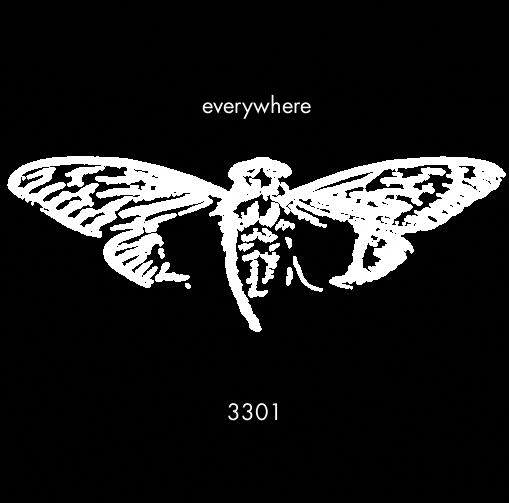
\includegraphics[scale=0.3]{agrippa}
	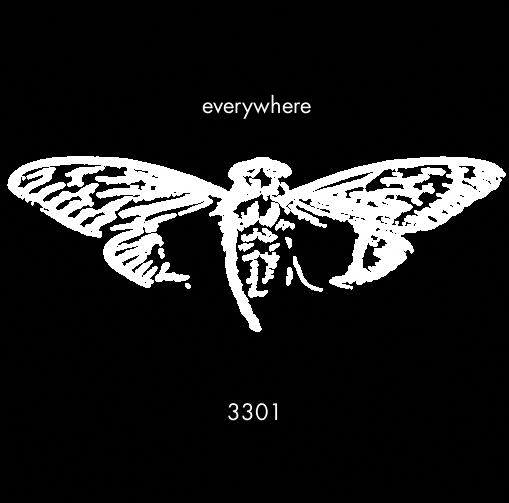
\includegraphics[scale=0.3]{brittanica}
	
	\caption{The two "everywhere" images}
\end{figure}

While they looked exactly the same, a different PGP-signed message was steganographically hidden within each variant.

\begin{figure}[h]
	\centering
	\tiny

	\begin{minipage}{0.5\textwidth}
		\verbatiminput{data/agrippa.asc}	
	\end{minipage}%
	\begin{minipage}{0.5\textwidth}
		\verbatiminput{data/brittanica.asc}
	\end{minipage}

	\caption{The two PGP-signed messages found}
\end{figure}
\FloatBarrier

The poems found in these messages hinted the book needed to complete the associated book code. For respectively each of the message above, they were "\textit{Agrippa (A Book of the Dead)}" by William Gibson and the "\textit{Encyclop\ae{}dia Brittanica}".

When deciphered, each book code led to an Tor address, allowing for further progress. \\

Unfortunately, the two "Everywhere" variants weren't properly archived.

The furthest archive of the "Agrippa" variant can be found on the wiki, added by Lurker69 in 2014 : \href{https://static.wikia.nocookie.net/uncovering-cicada/images/c/cd/Everyehere.jpg}{everywhere}.

For many years, no copy of the "Brittanica" variant was known. One copy recently surfaced when optimisticninja's gitlab repository was made public%
%
\footnote{\url{https://gitlab.com/optimisticninja/cicada3301/}, \texttt{2012/03.subreddit/04.qr\_codes}\\
	Archive :  \url{https://github.com/cicada-solvers/optimisticninja_cicada3301}}%
%
. No source that could justify where it originates from is provided. Furthermore, this same repository is known to contain fake assets, such as a fake screenshot of the countdown found on \texttt{845145127.com}. \\

This analysis aims at investigating the two archives of the "everywhere" to try to determine whether or not they are legitimate.

\section{Goals and methodology}

The upstream Outguess version in 2012 was Outguess v0.2. For this reason, we'll use its source code as the base of our analysis. \href{https://fossies.org/linux/privat/old/outguess-0.2.tar.gz/}{Source code}.

\section{Inner workings of Outguess}

\subsection{General principles}

To steganographically hide a message in an image, Outguess follows a serie of general steps. They have been highlighted in Outguess' \texttt{main} function, simplified below:

\begin{minted}[fontsize=\footnotesize]{C}
int
main(int argc, char **argv)
{
	// ...
	
	/* read command line arguments */
	while ((ch = getopt(argc, argv, "eErmftp:s:S:i:I:k:d:D:K:x:F:")) != -1)
		// ...
	}
	
	// `doretrieve` corresponds to the flag -r
	
	
	argc -= optind;
	argv += optind;
	
	// ...
	
	if (argc == 2) {
		srch = get_handler(argv[0]);
		if (srch == NULL) {
			fprintf(stderr, "Unknown data type of %s\n", argv[0]);
			exit (1);
		}
		if (!doretrieve) {
			// expect the second argument to be the output image name
			
			dsth = get_handler(argv[1]);
			if (dsth == NULL) {
				fprintf(stderr, "Unknown data type of %s\n",
				argv[1]);
				exit (1);
			}
		}
		fin = fopen(argv[0], "rb");
		// ...
		fout = fopen(argv[1], "wb");
		// ...
	} else {
		// read/write from stdin/stdout
		// ...
	}
	
	/* Initialize Golay-Tables for 12->23 bit error correction */
	// ...
	
	fprintf(stderr, "Reading %s....\n", argv[0]);
	image = srch->read(fin);
	
	if (extractonly) {
		// Special mode, only available iif the outguess executable is named "extract"
		// Usage : extract image.jpg output_file.txt
		
		int bits;
		/* Wen extracting get the bitmap from the source handler */
		srch->get_bitmap(&bitmap, image, STEG_RETRIEVE);
		
		fprintf(stderr, "Writing %d bits\n", bitmap.bits);
		bits = htonl(bitmap.bits);
		fwrite(&bits, 1, sizeof(int), fout);
		fwrite(bitmap.bitmap, bitmap.bytes, sizeof(char), fout);
		exit (1);
	} else if (doretrieve)
		// -r

		/* Wen extracting get the bitmap from the source handler */
		srch->get_bitmap(&bitmap, image, STEG_RETRIEVE);
	else {
		/* Initialize destination data handler */
		dsth->init(param);
		/* When embedding the destination format determines the bits */
		dsth->get_bitmap(&bitmap, image, 0);
	}
	fprintf(stderr, "Extracting usable bits:   %d bits\n", bitmap.bits);
	
	// -e
	if (doerror)
		cfg1.flags |= STEG_ERROR;
	
	if (!doretrieve) {
		// hide message in image

		// -m
		if (mark)
			cfg1.flags |= STEG_MARK;

		// -F ('on' by default)
		if (foil) {
			dsth->preserve(&bitmap, -1);
			
			if (bitmap.maxcorrect)
				fprintf(stderr,
					"Correctable message size: %d bits, %0.2f%%\n",
					bitmap.maxcorrect,
					(float)100*bitmap.maxcorrect/bitmap.bits);
		}
		
		do_embed(&bitmap, data, key, strlen(key), &cfg1, &cumres);
		
		// outguess can embed up to two messages (a key has to be used for the second message though)
		if (key2 && data2) {
			// ... embed the second file
		}
		
		if (foil) {
			// ...
			
			memset(steg_offset, 0, sizeof(steg_offset));
			steg_foil = steg_foilfail = 0;
			
			for (i = 0; i < bitmap.bits; i++) {
				if (!TEST_BIT(plocked, i))
				continue;
				
				cbit = TEST_BIT(pbits, i) ? 1 : 0;
				
				if (cbit == (data[i] & 0x01))
				continue;
				
				n = bitmap.preserve(&bitmap, i);
				if (n > 0) {
					/* Actual modificaton */
					n = abs(n - i);
					if (n > MAX_SEEK)
					n = MAX_SEEK;
					
					steg_offset[n - 1]++;
				}
			}
			
			/* Indicates that we are done with the image */
			bitmap.preserve(&bitmap, bitmap.bits);
			
			/* Calculate statistics */
			// ... mean
			// ... stddev
			
			fprintf(stderr, "Foiling statistics: "
				"corrections: %d, failed: %d, "
				"offset: %f +- %f\n",
				steg_foil, steg_foilfail,
				mean, sqrt(dev / (count - 1)));
		}
		
		fprintf(stderr, "Total bits changed: %d (change %d + bias %d)\n",
			cumres.changed + cumres.bias,
			cumres.changed, cumres.bias);
		fprintf(stderr, "Storing bitmap into data...\n");
		
		dsth->put_bitmap (image, &bitmap, cfg1.flags);
		
		#ifdef FOURIER
		// -f
		if (dofourier)
			fft_image(image->x, image->y, image->depth, image->img);
		#endif /* FOURIER */
		
		fprintf(stderr, "Writing %s....\n", argv[1]);
		dsth->write(fout, image);
	} else {
		/* Initialize random data stream */
		arc4_initkey(&as,  "Encryption", key, strlen(key));
		tas = as;
		
		iterator_init(&iter, &bitmap, key, strlen(key)); 
		
		encdata = steg_retrieve(&datalen, &bitmap, &iter, &as,
		cfg1.flags);
		
		data = decode_data(encdata, &datalen, &tas, cfg1.flags);
		free(encdata);
		
		fwrite(data, datalen, sizeof(u_char), fout);
		free(data);
	}
	
	// ...
	
	return 0;
}
\end{minted}

To hide a message \texttt{data} in the image file \texttt{a} to the output file \texttt{b}, the steps are as follows:
\begin{itemize}
	\item Detect the file format of \texttt{a} based on its file extension. As of Outguess v0.2, the following file formats are supported:
		\begin{itemize}
			\item JPEG files : \texttt{.jpg}
			\item PNM files : \texttt{.ppm}\footnote{Code exists to parse PNM files, but Outguess will not recognize the \texttt{.pnm} file extension. \\ PNM stands for "Portable anymap", a superset of PPM files: "Portable pixmap". They will be noneless be always refered to as PNM files below.}
		\end{itemize}
	
		Based on the detected file format, specialized function will be used. The \texttt{get\_handler} is used to return a structure encapsulating the function pointers: \texttt{handler}. It is defined as (C++-style comments have been added for additional information):
		
		\begin{minted}[fontsize=\footnotesize,escapeinside=||]{C}
typedef struct _handler {
	// Used to detect the file format
	char *extension;        /* Extension name */
	// Initialize the handler.
	// Will be called once for the handler used to output the file.
	// The parameter passed as argument can be set using -p
	//  (defaults to NULL)
	//
	// For the JPG handler, this parameter specifies the output
	//  quality. It's unused for the PNM handler.
	void (*init)(char *);
	// Parse the file handle and return an image object.
	image *(*read)(FILE *);
	// Write the image object to the file handle
	void (*write)(FILE *, image *);
	// Get the bitmap associated with the image.
	// The flag "STEG_RETRIEVE" will be passed as the last argument
	//  when the bitmap will be used to retrieve an embedded message.
	void (*get_bitmap)(bitmap *, image *, int);
	// Modify the image to match the changes made to its bitmap.
	// When -m is used, the flag STEG_MARK will be passed.
	void (*put_bitmap)(image *, bitmap *, int);
	// Callback to modify the file format handler that the bit at the
	//  offset given in the second parameter was flipped in the bitmap.
	// The purpose of this function is to preserve *some* statistics
	//  by modifying another part of the bitmap to cancel a given
	//  bitflip made.
	// It returns the index of the bit that was modified, if any, -1
	//  otherwise.
	//
	// Two offsets have a special meaning :
	//  - -1: the function is called once with this offset. It's used
	//      to signal to the statistics foiling logic to initialize.
	//     
	//      The code is expected to configure the bitmap's `preserve`
	//       function pointer|\footnotemark|, and its `maxcorrect` value if possible.
	//  - any offset greater or equal to the number of bitmap bits:
	//     Used to signal to the statistics foiling code to finish
	//      processing as the image will soon be written to disk.
	int (*preserve)(bitmap *, int);
} handler;
		\end{minted}

\footnotetext{The PNM handler's \texttt{preserve} is stubbed-out, meaning this file format does not support statistical foiling. However it does not initialize the \texttt{preserve} function pointer of the bitmap. This results will in a crash, meaning that to get Outguess to output an PNM file, statistical foiling had to be disabled.}

		The handlers for JPEG and PNM are respectively implemented in \texttt{jpg.c} and \texttt{pnm.c}. \\

		Two important structures are used: \texttt{image} and \texttt{bitmap}. \texttt{image} is defined as (C++-style commented have been added for additional information)\footnote{An additional unused \texttt{flags} field is also defined.}:
		\begin{minted}[fontsize=\footnotesize]{C}
typedef struct _image {
	// x: image width in pixels
	// y: image height in pixels
	// depth: number of color components
	// max: maximum value that a color component can be.
	//      (always 255 for JPEG)
	int x, y, depth, max;
	// pixels data. allocation of width * height * components bytes,
	//  filled with pixel colors components.
	u_char *img;

	// JPEG specific field: the bitmap of the image.
	// it is left uninitialized for PNM files.
	// this field exists only because of poor code design in my opinion,
	//  see the discussion below about STEG_RETRIEVE for more
	//  information
	bitmap *bitmap;
} image;
		\end{minted}

		The \texttt{read} function pointer of the \texttt{handler} structure can be used to return an \texttt{image} structure from a file handle. \texttt{write} can be used to write an \texttt{image} structure to a file. \\

		The \texttt{bitmap} structure represents the image data bits and is used during as an intermediary during the embedding process. It's defined as:
		\begin{minted}[fontsize=\footnotesize]{C}
typedef struct _bitmap {
	// array where each element represents 8 bits of data.
	u_char *bitmap;   /* the bitmap */
	// array where each bit represents a boolean value indicating
	//  whether the corresponding  bit in `bitmap` is currently in
	//  use to store some message data.
	u_char *locked;   /* bits that may not be modified */
	// array where each bit represents a boolean value indicating
	//  whether the corresponding bit in `bitmap` is currently in
	//  use to foil statistics.
	u_char *metalock; /* bits that have been used for foil */
	// TODO
	char *detect;   /* relative detectability of changes */
	// array where the ith element corresponds to the original data byte
	//  from where the ith bit of the bitmap comes from.
	char *data;   /* data associated with the bit */
	// number of allocated bytes for the `bitmap`, `locked` and
	//  `metalock` fields. equals to (bits + 7) / 8
	int bytes;    /* allocated bytes */
	// number of bits stored in the bitmap.
	int bits;   /* number of bits in here */
	
	// function set by the file format handler. It is used exactly
	//  as the handler's `preserve` function.
	/* function to call for preserve stats */
	int (*preserve)(struct _bitmap *, int);
	// length of embdeddable message in bits. Stands for unlimited
	//  when 0.
	size_t maxcorrect;
} bitmap;
		\end{minted}

		The handler function \texttt{get\_bitmap} is used to return the \texttt{bitmap} structure associated with a passed \texttt{image} structure. Then, the bitmap will be modified to embed the data. Once modified, the image is to be modified back to match the bitmap changes through the \texttt{put\_bitmap} function of the handler.
		
		Both functions have an additional \texttt{flags} parameter to specify additional behaviours. The flags can be:
		\begin{description}
			\item[for \texttt{get\_bitmap}: ] \texttt{STEG\_RETRIEVE}: flag present when the bitmap will be used to retrieve some data, rather than for embedding a file.
			
				This flag is unused for the PNM file format. For JPEG files, it is needed because the bitmap bits are based on DCT coefficients and not directly on pixels color components values. Thus, the bitmap to use when retrieving an embedded message is directly the bitmap encoded in the JPEG file. However, when producing a bitmap from an arbitrary \texttt{image} structure to be used to embed data, we don't have necessarily a bitmap of DCT coefficients to work with. Outguess solve this issue by always generating a bitmap from DCT coefficients by running the JPEG compression algorithm on the image pixel colors.
				
				We wouldn't want to compress the image data into a bitmap when simply retrieving data from an JPEG image as this could destroy the embedded data.

			\item[for \texttt{put\_bitmap}: ] \texttt{STEG\_MARK}: flag present when the option \texttt{-p} is used. In theory this should mark visually pixels holding embedded data, however this feature is only implemented for the PNM format handler.
			
				For this file format, it sets any pixel component having a bit changed to 255\footnote{regardless of the value of \texttt{max} -- this is a bug. Furthermore, Outguess can produce PPM files having pixels whose value are greater than the maximum field of their header.}.
		\end{description}

	\item Read the input file \texttt{a} into an \texttt{image} structure using its handler's \texttt{read} function.
	
	\item Initializes the output format handler by calling its \texttt{init} function.
	
	\item Get the output image bitmap, using image data of the input \textbf{a} we just generated. The \texttt{STEG\_RETRIEVE} flag isn't used there.

	\item If statistical foiling is enabled (it is by default), the handler's statistical foiling system is initialized by calling its \texttt{preserve} function on the bitmap, passing in the offset $-1$.
	
	\item The first data file is embedded, with the user-supplied key (defaults to "\texttt{Default key}")

	\item If supplied, the second data file is embedded.
	
	\item Is statistical foiling is enabled, the handler \texttt{preserve} function will be called with the offset of all bits that have actually been flipped. To do so, Outguess loops over all bitmap bits, skipping not locked bits (since these bits don't hold any information) and skipping bits left unchanged even though they are used to store information:
		\begin{minted}[fontsize=\footnotesize]{C}
      // statistics
      memset(steg_offset, 0, sizeof(steg_offset));
      steg_foil = steg_foilfail = 0;

      for (i = 0; i < bitmap.bits; i++) {
        // skip bits that don't hold any message bits
        if (!TEST_BIT(plocked, i))
          continue;
       	
        // skip unchanged bits
        cbit = TEST_BIT(pbits, i) ? 1 : 0;
        if (cbit == (data[i] & 0x01))
          continue;
	
        n = bitmap.preserve(&bitmap, i);

        // statistics
        if (n > 0) {
          /* Actual modificaton */
          n = abs(n - i);
          if (n > MAX_SEEK)
            n = MAX_SEEK;

          steg_offset[n - 1]++;
        }
      }
		\end{minted}

		The value returned by \texttt{preserve} in this case corresponds to the index of the bit that was changed to preserve the statistics, if any. If no bit was changed, a negative or null value is returned \footnote{If the modified offset was $0$, it wouldn't be counted in the foiling statistics. This is a bug.}. The \texttt{steg\_offset} array is only used to display the mean/standard deviation of the distance of changed bits to foil statistics \footnote{The final call to \texttt{preserve} will also try to modify some bits to preserve the distribution of DCT coefficients that failed to be preserved in previous calls. But these final modifications don't be taken into account in the displayed statistics. This is a bug.}.

		Finally, the statistical foiling logic is notified that the image finished being processed by calling the \texttt{preserve} function passing an offset greater or equal to the number of bits:
		\begin{minted}[fontsize=\footnotesize]{C}
      /* Indicates that we are done with the image */
      bitmap.preserve(&bitmap, bitmap.bits);
		\end{minted}
	
		During this entire process, the global variables are used to count the numbers of successful foils (\texttt{steg\_foil}) and unsucessful foils (\texttt{steg\_foilfail}). These variables are modified in handler-specific code. They are only used for informational purpose.
	
	\item The output \texttt{image} is synced with its bitmap. This takes into account all changes made to the bitmap.
	
	\item If the option \texttt{-f} has been compiled in Outguess (it's not by default) and if the user used it (it's not on by default), the image is outputed in frequency-space. The conversion is handled by the function \texttt{fft\_visible} implemented in \texttt{fourier.c}.
	
	\item The image is written to disk.
	
		
\end{itemize}

\subsection{JPG implementation}

For JPEG files, the generation of the bitmap is quite complicated. Outguess uses a patched version of the JPEG 6b library. This patched version\footnote{Note that the \texttt{.diff} file for the JPEG 6b library found in the Outguess source doesn't correspond to the patched source code.} hooks into the library internals and proxies reading/writing of the DCT coefficients.

The function that serves as the proxy can be found in \texttt{jpg.c}: \texttt{steg\_use\_bit}. It gets called whenever the JPEG library needs to store a DCT coefficient for a JPEG block. Changes to \texttt{jpeg-6b-steg/jcdctmgr.c}:
\begin{minted}[fontsize=\footnotesize]{C}
	// ...

	// replaced
	output_ptr[i] = (JCOEF) temp;
	// with
	output_ptr[i] = steg_use_bit(temp);

	// ...
\end{minted}
And to \texttt{jpeg-6b-steg/jdcoefct.c}:
\begin{minted}[fontsize=\footnotesize]{C}
	// ...

	// added
	/* Retrieve LSB from DCT coefficient */
	JBLOCKROW block = coef->MCU_buffer[blkn + xindex];
	int k;
	for (k = 0; k < DCTSIZE2; k++)
		steg_use_bit((JCOEF) (*block)[k]);

	// ...
\end{minted}

The \texttt{steg\_use\_bit} function is as follows (C++-style comments have been added for additional information, some unimportant lines have been omitted):
\begin{minted}[fontsize=\footnotesize]{C}
short
steg_use_bit (unsigned short temp)
{
	// only select coefficients where changing the LSB won't be too noticeable.
	// this skips DCT coefficients equal to 0 or 1
	if ((temp & 0x1) == temp)
		goto steg_end;
	
	switch (jpeg_state) {
		case JPEG_READING: // we're decoding a JPEG file
			// fill the bitmap
			WRITE_BIT(tbitmap.bitmap, off, temp & 0x1);
			tbitmap.data[off] = temp;

			// ...		
		
			off++;
		
			if (off >= tbitmap.bits) {
				// ... reallocate larger buffers
			}
			break;

		default: // JPEG_WRITING, we're writing a JPEG file out to disk
			// overwrite LSB of the coefficient
			temp = (temp & ~0x1) | (TEST_BIT(tbitmap.bitmap, off) ? 1 : 0);
			off++;
		
			break;
	}

  steg_end:
	// ...
	
	return temp;
}
\end{minted}

\subsection{Statistical foiling}

Outguess version 0.2 introduced new methods that made it undetectable to statistical tests known when it was released\cite{def01}. These methods are known as "statistical foiling" in Outguess' source code. 

Most statistics to detect the use of steganography in JPEG images relied on the analysis of the distribution of JPEG DCT coefficients. As most methods to steganographically hide a message in a JPEG image do so in the least-significant bits (LSBs) of DCT coefficients, it can be assumed that the frequency of adjacent coefficients will be more similar than in an unmodified image. Thus, attacks analysed properties of the distribution of DCT coefficients across an image \cite{det01}.

To make Outguess v0.2 undetectable using these methods, it now made sure to keep the distribution of DCT coefficients intact when embedding a message \cite{def01}. A new correction step would now run after the message was embedded. Its purpose was to modify some DCT coefficients that haven't yet been used to match the original DCT distribution.

\subsubsection{Maximum message length}

Because some bits would now be needed to correct the DCT distribution, computing the maximum embeddable message length isn't as straightforward \cite{def01}\cite{att02}. Consider a JPEG image. Its DCT coefficients can range from $-127$ to $128$. Let $h_i$ be the number of DCT coefficients with the value $i$ ($-127 \le i \le 128$). In other words, $(h_i)_{-127 \le i \le 128}$ is the histogram of the DCT coefficients. Let $P = \sum_{i = -127}^{128} h_i - h_0 - h_1$ be the number of coefficients considered. We'll denote $f_i = \frac {h_i} P$ as the frequency of coefficient with the value $i$.

Consider a message of $m$ bits. Embedding it in the image will modify the LSB of $m$ DCT coefficients at random. However, the LSB of a given coefficient will sometimes already be the corresponding bit in the message $m$: on average, this will happen 1 times out of 2. That is to say, $\frac m 2$ DCT coefficients will on average be actually modified after embedding the message.

Let $i \in \{-127, \ldots, 128\}$. If a coefficient with value $i$ is modified, its new value will be $i \oplus 1$, that is to say $2k + 1$ if $i = 2k$, $2k$ otherwise. After embedding the message, the updated frequencies for the values $2k$ and $2k + 1$ are: \[
	\begin{aligned}
		f_{2k}^\star &= \frac {h_{2k}^\star} P = \frac {h_{2k} - \frac m 2 h_{2k} + \frac m 2 h_{2k + 1}} P \\
		&= f_{2k} - \frac 1 2 \frac m P \left( f_{2k} - f_{2k + 1} \right)		
	\end{aligned}
\]\[
	\begin{aligned}
		f_{2k + 1}^\star &= \frac {h_{2k + 1}^\star} P = \frac {h_{2k + 1} - \frac m 2 h_{2k + 1} + \frac m 2 h_{2k}} P \\
		&= f_{2k + 1} + \frac 1 2 \frac m P \left( f_{2k} - f_{2k + 1} \right)
	\end{aligned}
\]

How many coefficients with the value $i$ are holding data of the message? $m f_i$ are (even though on average for half of these coefficients their LSB stayed the same, simply because they already matched the bits of the message). We will thus have $h_i - m f_i$ coefficients with the value $i$ remaining for the correction step.

In the correction step, we want to use some of those bits to change the modified frequencies $f^\star$ back to their original values $f$. The (possibly negative) number of DCT coefficients with value $2k$ to purposely change to $2k + 1$ is the average of the difference in distribution between values $2k$ and $2k + 1$: \[
	\begin{aligned}
		\delta_k &= \frac {(h_{2k} - h_{2k+1}) - (h^\star_{2k} - h^\star_{2k + 1})} 2	\\
			&= P \times \frac {(f_{2k} - f_{2k+1}) - (f^\star_{2k} - f^\star_{2k + 1})} 2	\\
			&= P \times \frac 1 2 \frac {2m} {2P} \left(f_{2k} - f_{2k + 1}\right) \\
			&= P \times \frac 1 2 \frac m P \left(f_{2k} - f_{2k + 1}\right)
	\end{aligned}
\]

Thus, at least $\left|\delta_k\right|$ bits are needed for the coefficient $2k$ if $f_{2k} > f_{2k + 1}$, for the coefficient $2k + 1$ otherwise. This results in the following inequality: \[
	\forall k, \left|\delta_k\right| \le \min(h_{2k} - m f_{2k}, h_{2k + 1} - m f_{2k + 1})
\]

Or \[
	P \times \frac 1 2 \frac m P \left|f_{2k} - f_{2k + 1}\right| \le P \times \left(1 - \frac m P\right) \min(f_{2k}, f_{2k + 1})
\] \[
	\frac 1 2 m \left|f_{2k} - f_{2k + 1}\right| \le \left(P - m\right) \min(f_{2k}, f_{2k + 1})
\]

Finally, we can get an inegality on the message size $m$ : \[
	m \le \frac { P \times \min(f_{2k}, f_{2k + 1}) } { \frac 1 2 \left|f_{2k} - f_{2k + 1}\right| + \min(f_{2k}, f_{2k + 1}) }
\]

With $f_k = \max(f_{2k}, f_{2k + 1})$ and $\overline f_k = \min(f_{2k}, f_{2k + 1})$, this simplifies to : \[
	m \le 2 P \times \frac {\overline f_k} { f_k + \overline f_k }
\]

This relation should hold for all $k$ different than $0$ (as DCT coefficients $0$ and $1$ are ignored). \\

Code-wise, this computation happens in the first call of the JPEG handler's \texttt{preserve} function:
\begin{minted}[fontsize=\footnotesize]{C}
preserve_jpg(bitmap *bitmap, int off)
{
	char coeff;
	int i, a, b;
	char *data = bitmap->data;
	
	// Initialization call
	if (off == -1) {
		int res;
		
		// ...

		memset(dctfreq, 0, sizeof(dctfreq));
		
		// ...

		/* Calculate coefficent frequencies */
		for (i = 0; i < bitmap->bits; i++) {
			dctfreq[data[i] + 127]++;
		}
		
		a = dctfreq[-1 + 127];
		b = dctfreq[-2 + 127];
		
		if (a < b) {
			fprintf(stderr, "Can not calculate estimate\n");
			res = -1;
		} else
			res = 2*bitmap->bits*b/(a + b);
		
		// ...
		
		bitmap->maxcorrect = res;
		return (res);
	} else if (off >= bitmap->bits) {
		// ...

	//...
\end{minted}

Interestingly enough, Outguess does not check that this relation holds for all pairs of DCT coefficients, but only for the pair $(-1, -2)$. Furthermore, it will exit when $h_{-2} > h_{-1}$ as it fails to "calculate an estimate". {\color{red} TODO: Why?}

\subsubsection{Outguess' statistical foiling algorithm}

Furthermore, this piece of logic in \texttt{preserve\_jpg} also initializes the statistical foiling logic (omitted in the previous code snippet -- C++-style comments have been added to give additional information).

The JPEG statistical foiling implemented in Outguess is a variation of Algorithm 1 from Provos' \cite{def01}.

The global variable \texttt{dctfreq} is an array of threshold frequencies for each coefficient value. From \cite{def01}: "The threshold indicates how many errors in the histogram we are willing to tolerate for a specific DCT coefficient. [...]. When the number of errors for a coefficient exceeds its threshold, we modify the image to preserve the statistics for that coefficient." In \cite{def01} it is named $N^\ast$.

The global variable \texttt{dctadjust} keeps track of the number of DCT coefficients that have to be changed for each coefficient value in order to keep the coefficient distribution intact. In \cite{def01}, this array is named $N_{error}$. \footnote{A third global variable \texttt{dctpending} keeps track of the total number of pending coefficient changes. However it stands unused.}

\begin{minted}[fontsize=\footnotesize]{C}
preserve_jpg(bitmap *bitmap, int off)
{
	char coeff;
	int i, a, b;
	char *data = bitmap->data;
	
	// Initialization call
	if (off == -1) {
		int res;
		
		// ... debug output
		
		// initialize the bitmap `preserve` function, as required
		bitmap->preserve = preserve_jpg;
		// so far, no bits have been used for statistics foiling.
		memset(bitmap->metalock, 0, bitmap->bytes);
		
		// no coefficients have to be adjusted for now
		memset(dctadjust, 0, sizeof(dctadjust));

		// threshold frequencies computation: step 1 of Algorithm 1
		memset(dctfreq, 0, sizeof(dctfreq));
		// ...
		
		/* Calculate coefficent frequencies */
		for (i = 0; i < bitmap->bits; i++) {
			dctfreq[data[i] + 127]++;
		}
		
		// ...

		/* Pending threshold based on frequencies */
		for (i = 0; i < DCTENTRIES; i++) {
			// step 2. of Algorithm 1
			dctfreq[i] = dctfreq[i] /
				((float)bitmap->bits / DCTFREQRANGE);
			dctfreq[i] /= DCTFREQREDUCE;

			// differents from Algorithm 1
			if (dctfreq[i] < DCTFREQMIN)
				dctfreq[i] = DCTFREQMIN;
	
			// ... debug output
		}
		
		// ...
		return (res);
	} else if (off >= bitmap->bits) {
		// ...
		
	//...
\end{minted}

Note the presence of an additional step, where the threshold frequencies are capped at a minimum. \\

The logic ran when the image finishes processing is a direct implementation of Algorithm 1's last step \cite{def01}:
\begin{minted}[fontsize=\footnotesize]{C}
	/* Reached end of image */
	for (i = 0; i < DCTENTRIES; i++) {
		while (dctadjust[i]) {
			dctadjust[i]--;
		
			coeff = i - 127;
		
			if (preserve_single(bitmap, bitmap->bits - 1,
					coeff) != -1)
				steg_foil++;
			else
				steg_foilfail++;
		}
	}
\end{minted}

The same can be said for the third case as to why \texttt{preserve\_jpg} might be called: to indicate that a bit was modified.
\begin{minted}[fontsize=\footnotesize]{C}
	// step 3
	/* We need to find this coefficient, and change it to data[off] */
	coeff = data[off] ^ 0x01;

	// step 4
	if (dctadjust[data[off] + 127]) {
		/* But we are still missing compensation for the opposite */
		dctadjust[data[off] + 127]--;
		// ...
		return (0);
	}
	
	// step 5
	if (dctadjust[coeff + 127] < dctfreq[coeff + 127]) {
		dctadjust[coeff + 127]++;
		// ...
		return (0);
	}
	
	// call to exchDCT
	i = preserve_single(bitmap, off, coeff);
	
	if (i != -1) {
		steg_foil++;
		return (i);
	}
	
	/* We have one too many of this */
	dctadjust[coeff + 127]++;
	// ...
	
	return (-1);
\end{minted}

Algorithm 2, \textit{exchDCT} is exactly implemented by the function \texttt{preserve\_single}.

\bibliographystyle{plain}
\bibliography{bibliography}

\end{document}
